\documentclass[12pt]{article}

\usepackage{sbc-template}
\usepackage{graphicx,url}
\usepackage[utf8]{inputenc}
\usepackage[brazil]{babel}
\usepackage{amsmath}
% \usepackage[latin1]{inputenc}  

\sloppy

\title{Trabalho Final \\ Sistemas Operacionais}

\author{Bruno Feitosa\inst{1}}

\address{Instituto de Ciências Matemáticas e de Computação -- Universidade de São Paulo
\email{feitosa.bruno@usp.br}
}

\begin{document} 

\maketitle

\begin{abstract}
This paper discuss and compares three different methods to calculate $\pi$,
one method to calculate Call prices on Stock Market options,
and how these methods can use POSIX PThreads to optimize these methods through parallelization.
\end{abstract}
     
\begin{resumo} 
Este artigo discute e compara três métodos diferentes para calcular $\pi$,
um método para calcular o valor de opções Call no Mercado de Ações,
e como estes métodos podem utilizar POSIX PThreads para otimizar estes métodos
através de paralelização.
\end{resumo}


\section{Resumo dos Algoritmos}

A seguir serão brevemente descritos os algoritmos usados neste trabalho.
Vale notar, que devido a estes algoritmo utilizarem números com tamanhos e precisões maiores
do que as padrões da linguagem de implementação, foram utilizadas duas bibliotecas,
a GNU Multiple Precision Library\cite{GNU:MP} e a
GNU Multiple Precision Floating point with correct Rounding Library\cite{GNU:MPFR}.

\subsection{Cálculo do $\pi$ - Método Gauss-Legendre}

Este algoritmo é uma aplicação da regra de quadratura Gauss-Legendre,
para aproximação numérica de uma integral definida.
O algoritmo se baseia em substituir dois números por suas médias aritméticas e geométricas,
para aproximá-las a média geométrica-aritméticas.\\
Para o cálculo do valor de $\pi$, é usada a função trigonométrica do $sen$ e o ângulo de $\pi/4$.

\subsection{Cálculo do $\pi$ - Método Bailey-Borwein-Plouffe}

O método Bailey-Borwein-Plouffe é baseado na fórmula BBP para o cálculo do $\pi$
\cite{Bailey:97}.
Sua vantagem está no fato de que todos os fatores da fórmula são múltiplos de 8,
o que acelera a computação em sistemas hexadecimais.

\subsection{Cálculo do $\pi$ - Método Monte Carlo}

O método de Monte Carlo é um método estocástico, que relaciona a área de um quadrado com lado
$2.R$ e a área de um círculo inscrito nele com raio $R$. Como a relação entre estas áreas é
$\pi$, a seleção aleatória de pontos dentro do quadrado tem $\pi$ vezes mais chance de caírem
dentro do círculo do que fora dele.

\subsection{Cálculo de Preços de Opções - Método Black-Scholes}

O método Black-Scholes é utilizado para se calcular Opções (\textit{Call} e \textit{Put}) de
Ações. Opções são derivativos de Ações, ou seja, são Ativos que dependem de um outro Ativo,
que nesse caso, é a Ação de referência da Opção. Como opções agem como contratos de Compra/Venda
dos Ativos de referência, seus preços estão ligados ao preço dos Ativos de referência e ao
estado do mercado em si. Como sua precificação não é tão direta como a negociação de Ações no
Mercado, método como o de Black-Scholes permitem uma melhor estimativa de seus preços.

\section{Metodologia dos Algoritmos e Discussões} \label{sec:formulas}

A seguir são explicitadas as fórmulas de cada algoritmo, assim como comentários a respeito sobre
condições intrínsecas de execução, particularidades, ou oportunidades de paralelização.

\subsection{Algoritmo Gauss-Legendre}

\begin{equation}
	\begin{aligned}
		a_{n+1} &= \frac{a_n + b_n}{2}			& a_0 &= 1\\
		b_{n+1} &= \sqrt{a_n b_n}				& b_0 &= \frac{1}{\sqrt{2}} \\
		t_{n+1} &= t_n - p_n(a_{n}-a_{n+1})^2	& t_0 &= \frac{1}{4} \\
		p_{n+1} &= 2p_n							& p_0 &= 1		
	\end{aligned}
\end{equation}
\begin{equation}
	\pi \approx \frac{(a_{n+1}+b_{n+1})^2}{4t_{n+1}}
\end{equation}

Devido a natureza sequencial do algoritmo (o passo seguinte usa o resultado do passo anterior),
sua paralelização não pode ser feita em relação a iteração, mas sim somente em relação aos quatro
fatores ($a$, $b$, $t$, e $p$). Dentre eles, $b_{n+1}$ possui a maior complexidade de cálculo,
por possuir o cálculo de uma raiz quadrada. Nenhuma das variáveis utilizadas no seu cálculo
será alterada durante a execução da iteração, então seu cálculo pode ser feito de forma
independente das restantes. O fator $a_{n+1}$ possui a segunda maior complexidade, e seria um
outro candidato a paralelização. Porém, o valor de $a_{n+1}$ é utilizado na iteração corrente
para o cálculo de $t_{n+1}$. Dessa forma, a mais interessante forma de paralelização deste
algoritmo está em paralelizar o cálculo de $b_{n+1}$ em relação ao cálculo de
$a_{n+1}$ e $t_{n+1}$. A escolha de calcular $p_{n+1}$ junto com $b_{n+1}$ ou
$a_{n+1}$ e $t_{n+1}$ é irrelevante devido a baixa complexidade da operação.

\subsection{Algoritmo Bailey-Borwein-Plouffe}

\begin{equation}
	\pi \quad = \quad \sum_{k=0}^{\infty}\left(\frac{1}{16^k}\right).
	\left(
		\frac{4}{8.k + 1} - \frac{2}{8.k + 4} - \frac{1}{8.k + 5} - \frac{1}{8.k + 6}
	\right)
\end{equation}
\begin{equation}
	\pi \quad = \quad \sum_{k=0}^{\infty} a_k.
	\left(p^1_k + p^2_k + p^3_k + p^4_k\right)
\end{equation}

Em contrapartida ao método Gauss-Legendre, o método BBP pode ser paralelizado tanto em iteração
(todas as iterações são independentes entre si) quanto em parcelas (os termos $a_k$ e $p^n_k$
são independentes entre si). Estas características, combinadas ao fato de que os fatores de
multiplicação são múltiplos de 8, demonstram a capacidade de execução rápida deste algoritmo.
Para este trabalho, foi feita a paralelização em parcelas (cada iteração calculou as parcelas
em paralelo).

\subsection{Algoritmo Monte Carlo}

\begin{figure}[h]
	\centering
	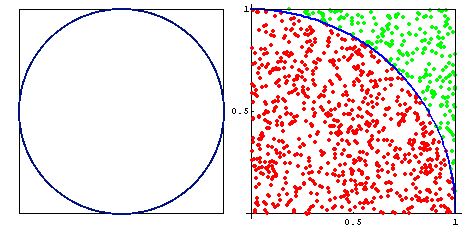
\includegraphics[width=.8\textwidth]{fig01.png}
	\caption{Visualização do Método de Monte Carlo}
	\label{fig:MonteCarloFig01}
\end{figure}
	
Para o método de Monte Carlo, cada ponto pode ser gerado e testado (se a soma de seus quadrados
é maior que 1) de forma completamente independente. Dessa forma, o algoritmo é paralelizável
a nível de iteração. A dificuldade da paralelização deste algoritmo está em relação a geração
de números aleatórios. 

\subsection{Algoritmo Black-Scholes}

\begin{equation}
	\begin{aligned}
		\mathtt{t}			&= S.e^{(r-\frac{v^2}{2}).T}.e^{(v.\sqrt{T}).randomNumber()}\\
		\mathtt{aux1}		&= S.e^{(r-\frac{v^2}{2}).T}\\
		\mathtt{aux2}		&= (v.\sqrt{T})\\
		\mathtt{trial[i]}	&= e^{-r.T}.\mathtt{max}(\mathtt{t}-E;0)\\
		\mathtt{aux3}		&= e^{-r.T}
	\end{aligned}
\end{equation}
\begin{equation}
	\mathtt{t}>E \quad ... \quad randomNumber() < \frac{ln(E/\mathtt{aux1})}{\mathtt{aux2}}
	\label{sec:validityCondition}
\end{equation}

Similar ao método de Monte Carlo, o método de Black-Scholes baseado em Monte Carlo gera $N$
testes com números aleatórios entre 0 e 1, e infere o resultado a partir de dados estocásticos.
Dessa forma, o algoritmo é paralelizável a nível de iteração. \\
Uma ressalva deste algoritmo é que ele não é válido para condições onde todos os números
aleatórios gerados não são capazes de satisfazer a condição de validade demonstrada
na Equação \ref{sec:validityCondition}, visto que todo teste $\mathtt{trial[i]}$ resultará em 0.

\section{Resultados}

A rápida convergência do algoritmo de método de Gauss-Legendre para o cálculo de $\pi$
foi observada pela forma como o resultado se tornava errôneo caso muitas iterações fossem feitas.
Estes erros surgiam do fato da parcela $t_n$ assumir valores além da precisão escolhida.
Os limites observados relacionados com a precisão escolhida podem ser observados na
Tabela \ref{tab:table01}.

\begin{table}[h]
\centering
\caption{Limite de Iterações e Precisão (em bits)}
\begin{tabular}{|c|c|}
	\hline
	Número de Iterações & Precisão (bits)\\
	\hline
	600		& 256\\
	1000	& 512\\
	2000	& 1024\\
	15000	& 8192\\
	\hline
\end{tabular}
\label{tab:table01}
\end{table}

Uma precisão com tamanho de 1MB causou um travamento na execução do programa.
Com o objetivo de estressar o algoritmo e a biblioteca, foi escolhida a precisão de 1KB.
Os tempos de execução do algoritmo não-paralelizado e paralelizado podem ser vistos na
Tabela\ref{tab:table02}

\begin{table}[h]
	\centering
	\caption{Limite de Iterações e Precisão (em bits)}
	\begin{tabular}{|l|c|c|}
		\hline
		{}		& Não Paralelizado & Paralelizado \\
		\hline
		user 	& 600	& 256\\
		system 	& 1000	& 512\\
		user 	& 2000	& 1024\\
		\hline
	\end{tabular}
	\label{tab:table02}
\end{table}
	

\bibliographystyle{sbc}
\bibliography{report}

\end{document}
